\section{Methods}
The experimentation process can be divided into three stages: 
\begin{enumerate}
    \item Electrode construction
    \item Battery assembly
    \item Evaluation process
\end{enumerate}

In total, seven individual variables are assessed, of which the cathode layer-thickness, anode carbon source and evaluation process, which includes the charge time and the discharge load, will be presented in more detail. The investigation of the titanium-dioxide powder used, the sodium-perchlorate concentration as well as the battery form factor will be briefly mentioned, however, they were evaluated as being less impactful on the battery effectiveness.

\subsection{Cathode Layer Thickness}
\subsubsection{Experiment Design}
The core substance comprising the cathode is titanium-dioxide, as it can effectively intercalate sodium-ions and is commonly used as both anodes and cathodes in sodium-ion batteries\cite{Guo2016}.
In essence, the cathode is made up of a FTO glass slide acting as the current collector, coated with a titanium-dioxide suspension, and left to sinter in a drying oven. Different thicknesses of titanium-dioxide layers are investigated, with the aim to create a conductive titanium-dioxide coating. The actual performance in a battery was not measurable during the experiment, as this part of the investigation was completed before an actual battery was constructed and acted as a precursor to the battery design process.

\subsubsection{Variables}
\begin{table}[h]
\renewcommand{\arraystretch}{1.3}
\caption{Iteration Parameters}
\label{table:parameterscathode}
\centering
\begin{tabular}{l|l|l||l}
\multicolumn{3}{c||}{\bfseries Parameter}&\bfseries Values\\
\hline
\hline
\multicolumn{2}{c|}{\multirow{2}{*}{Constant}}&The current collector&FTO slide\\
\cline{3-4}
\multicolumn{2}{c|}{}&The cathode substance&Titanium-dioxide\\
\hline\hline
\multirow{2}{*}{Varying}&Independent&The TiO$_2$ layer thickness&$\approx$\SI{1}{\mm}, $\approx$\SI{1.5}{\mm}, $\approx$\SI{2}{\mm}\\
\cline{2-4}
&Dependent&The conductivity of the TiO$_2$ layer&To be measured\\
\end{tabular}
\end{table}
            
\subsubsection{Process}
\begin{enumerate}
\item The FTO glass slides are cleaned using a general cleaning solution, followed by a glass specific cleaner.
\item A diluted nitric-acid solution is created by diluting \SI{1}{\ml} of a \SI{1}{\mol\per\L} nitric-acid solution with \SI{1000}{\ml} of de-ionized water. The dilution ratio is negligible, whereas a pH between 3-4 is critical.
\item Next, \SI{6}{\g} of Degussa titanium-dioxide powder is added to \SI{12}{\ml} of the diluted nitric-acid solution and crushed using a glass rod to ensure total suspension.
\item Subsequently, three FTO glass slides are prepared by taping off three of their sides with thin scotch tape. Approximately $3$ to \SI{4}{\mm} of each edge should be covered by tape.
\item Next, 1 droplet of the titanium-dioxide suspension is applied to the first slide with a single-use pipette. 2 droplets are applied to the second and 3 droplets to the third slide. The droplets are positioned on one of the taped-off sides between two strips of tape while touching the third.
\item The titanium-dioxide suspension is then spread over the entire surface of the FTO glass slide with a glass rod. As the rod is moved from side a to b it glides directly on top of the taped edges. Thus the thickness of the tape determines the pressure applied while spreading the suspension and therefore serves as a measure of layer thickness. It is recommended to swivel the glass rod right to left in the droplets prior to spreading the suspension, thus ensuring full coverage of the glass slide. The entire surface can be covered with a single motion, which results in a more even coating.
\item The coated slides are air-dried for \SI{10}{\minute}. The tape is removed and the slides are then placed in a drying oven to sinter at \SI{200}{\degreeCelsius} for another \SI{10}{\minute}.
\item Finally, the resistance between the FTO coating and the titanium-dioxide layer is measured with a multimeter. The first probe is placed directly upon the FTO coating on one of the open edges previously covered by tape, while the second is placed directly upon the titanium-dioxide layer.
\end{enumerate}
            
\begin{figure}[ht!]
\centering
\subfloat[]{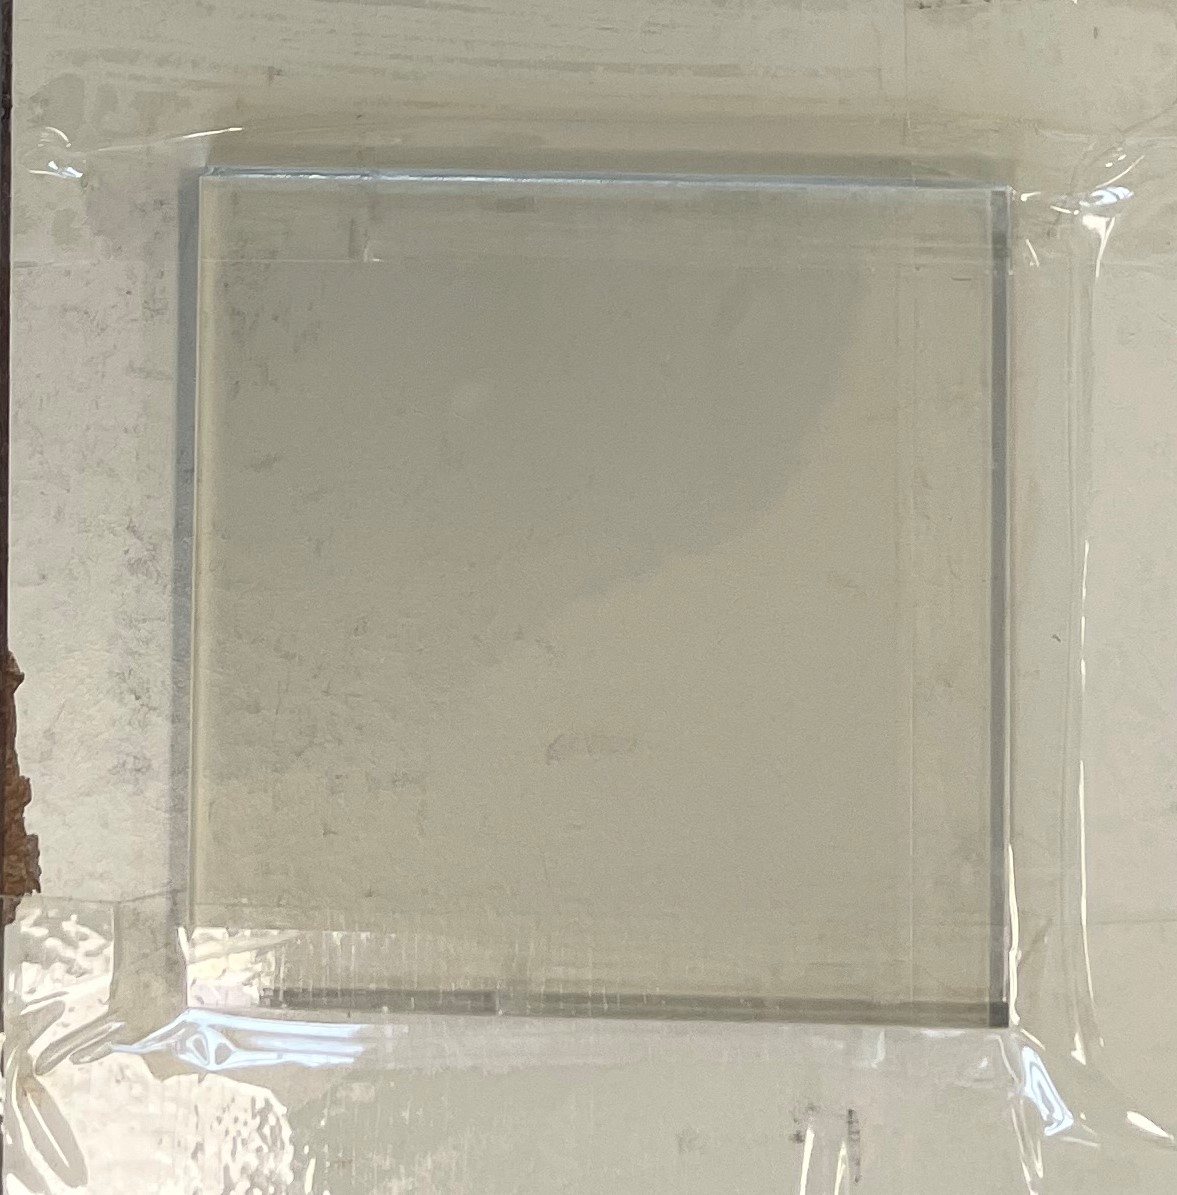
\includegraphics[width=0.331\textwidth]{taped_cathode.jpg}}
\subfloat[]{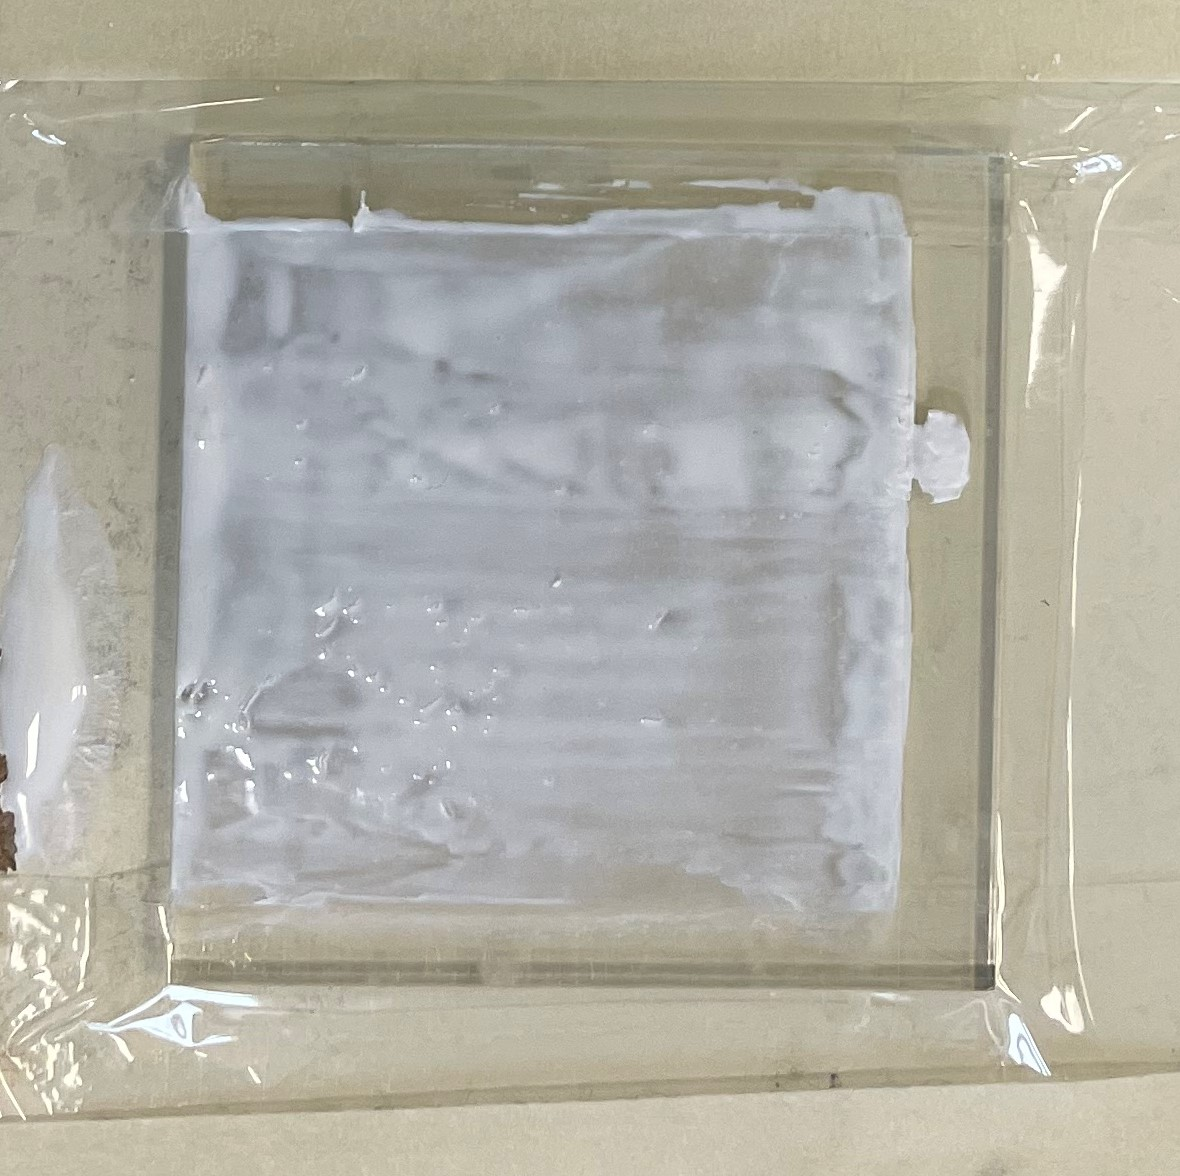
\includegraphics[width=0.338\textwidth]{coated_cathode.jpg}}
\subfloat[]{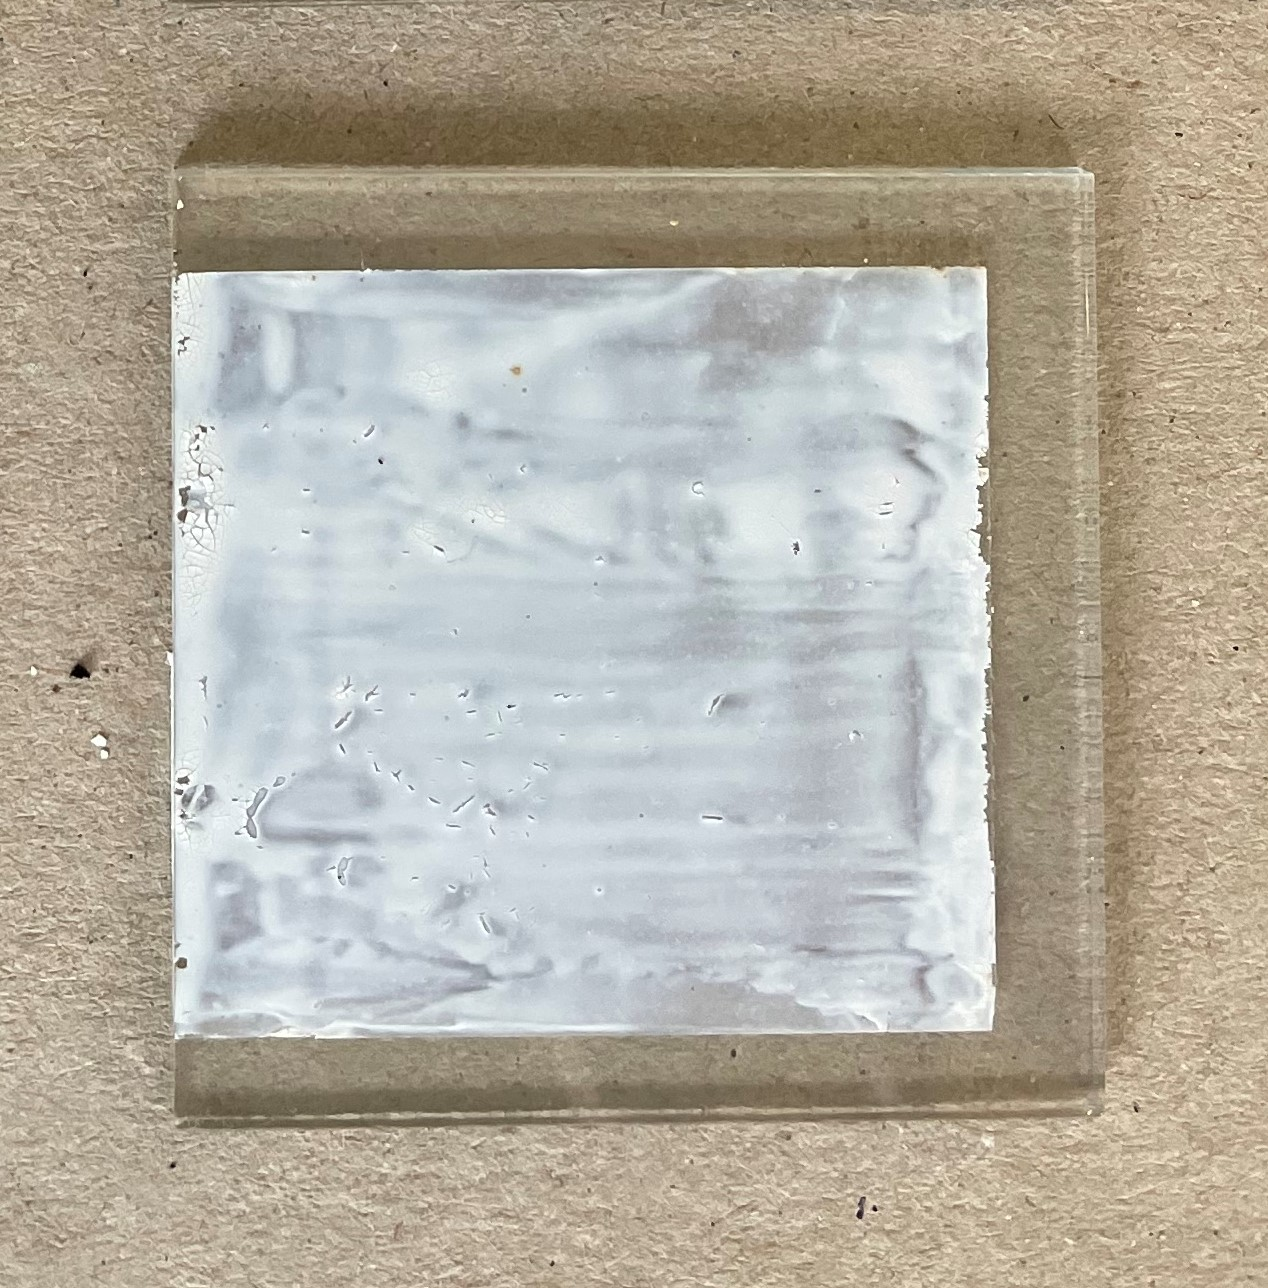
\includegraphics[width=0.331\textwidth]{final_cathode.jpg}}
\caption{(a): An FTO slide prepared by taping off three of the four sides. (b): An FTO slide after the titanium-dioxide coating. (c): The final cathode after sintering.}
\label{fig:cathodeprocess}
\end{figure}

\newpage

\subsection{Anode Carbon Source}
\subsubsection{Experimental Design} 
The anode is comprised of graphite, even though it is known that sodium-ions do not intercalate well in graphite and hard carbon should be used instead\cite{Xie2020}. However, since this experiment intercalates perchlorate ions in the graphite anode, this limitation can be disregarded. 
Three different sources of carbon are compared in terms of their use in a battery stack: An IKEA tea light candle, a Faber Castell pure graphite pencil and a laboratory grade graphite anode\cite{Ikea2022, Castell2022}.
The effectiveness is measured by determining the battery charge voltage, discharge voltage and peak discharge current over a \SI{1e3}{\ohm} resistance.

\subsubsection{Variables}
\begin{table}[h]
\renewcommand{\arraystretch}{1.3}
\caption{Iteration Parameters}
\label{table:parametersanode}
\centering
\begin{tabular}{l|l|l||l}
\multicolumn{3}{c||}{\bfseries Parameter}&\bfseries Values\\
\hline
\hline
\multicolumn{2}{c|}{\multirow{2}{*}{Constant}}&The current collector&FTO slide\\
\cline{3-4}
\multicolumn{2}{c|}{}&The anode substance&Carbon\\
\hline\hline
\multirow{2}{*}{Varying}&Independent&The carbon source&Graphite, soot, pencil\\
\cline{2-4}
&\multirow{2}{*}{Dependent}&The charged voltage in a battery&To be measured\\
\cline{3-4}
&&The discharge current in a battery&To be measured\\
\end{tabular}
\end{table}
    
\begin{figure}[ht!]
\centering
\subfloat{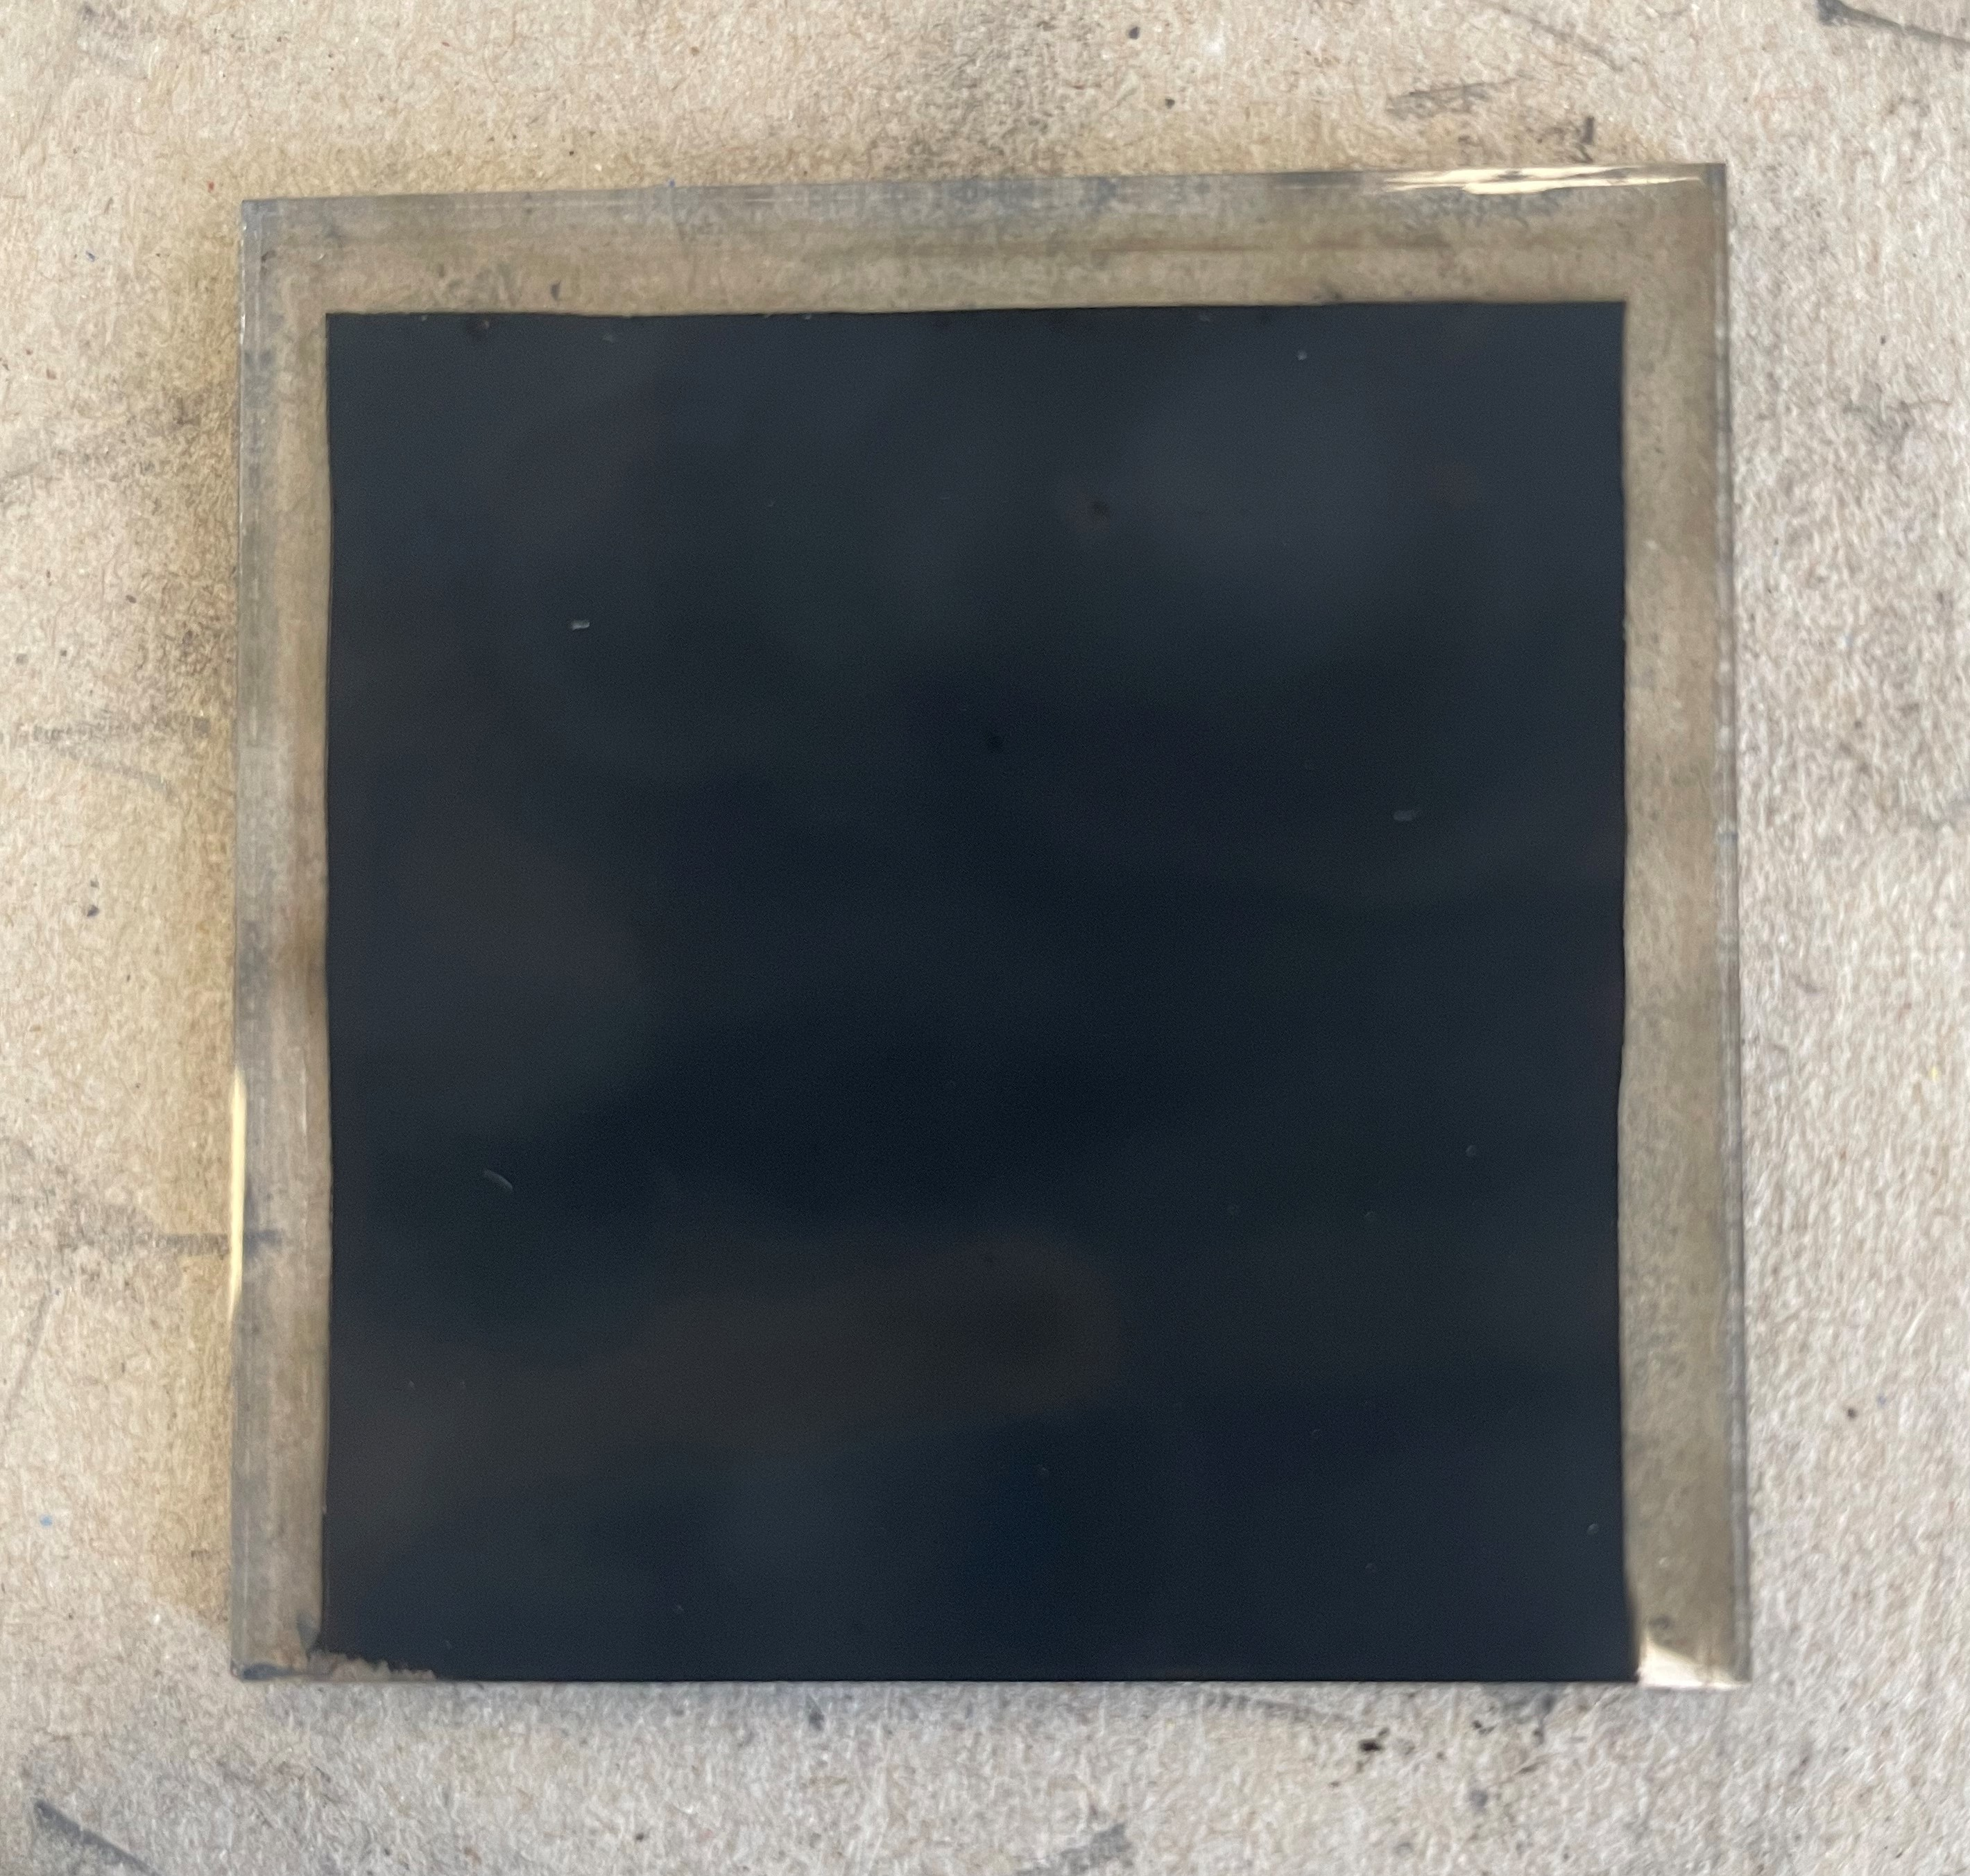
\includegraphics[width=0.427\textwidth]{soot_anode.jpg}}
\subfloat{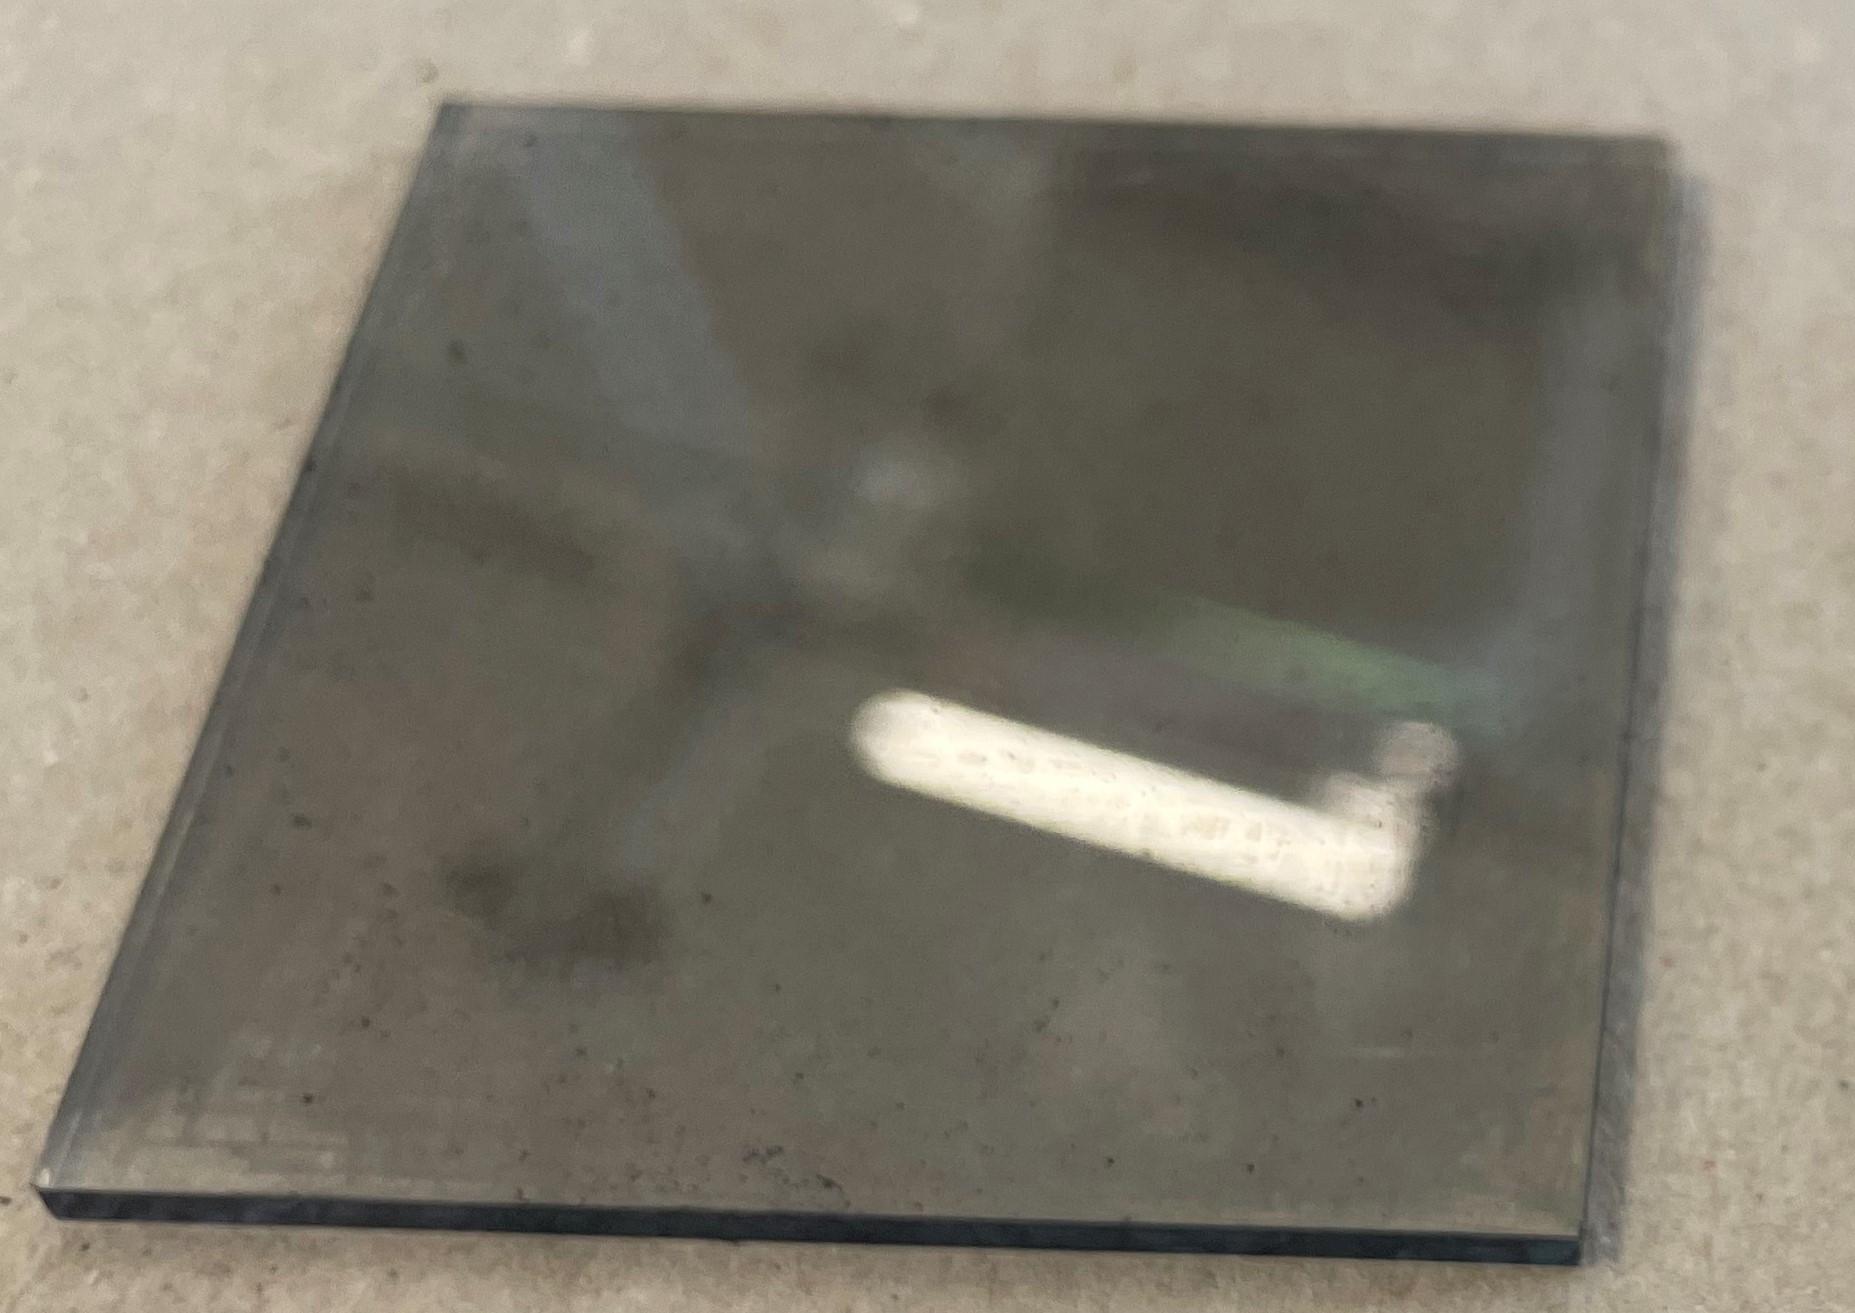
\includegraphics[width=0.573\textwidth]{graphite_anode.jpg}}
\caption{(a): FTO slide covered in candle soot. (b): FTO slide coated with a pure graphite pencil.}
\label{fig:anodefig}
\end{figure}
    
\subsubsection{Process}

\begin{enumerate}
\item First, the FTO glass slides are cleaned using a general cleaning solution, followed by a glass specific cleaner.
\item Next, the tea light candle used is lit beforehand to ensure a steady and even flame during the experiment.
\item Additionally, the laboratory grade graphite electrode is roughed up using 80 grit sandpaper, to remove any substances obstructing the surface.
\item Subsequently, the two FTO glass slides are prepared by taping off a single side on the first slide and three sides on the second slide. Approximately \SI{3}{\mm} of each edge are covered with tape.
\item The FTO glass slide with three taped-off sides is covered in soot, by passing it over the pre-lit candle multiple times in quick succession. The slide is held a few millimetres above the wick and is continuously passed over the flame until an even coating of soot is achieved.
\item The FTO glass slide with a single taped-off side is covered by a layer of graphite using the pure graphite pencil. It is continuously painted until a homogeneous gray color is achieved and no obvious stroke marks are visible.
\item Finally, the tape is removed, and the cathodes are tested in a battery setting. The battery layout is described below.
\end{enumerate}

\begin{figure}[ht!]
\centering
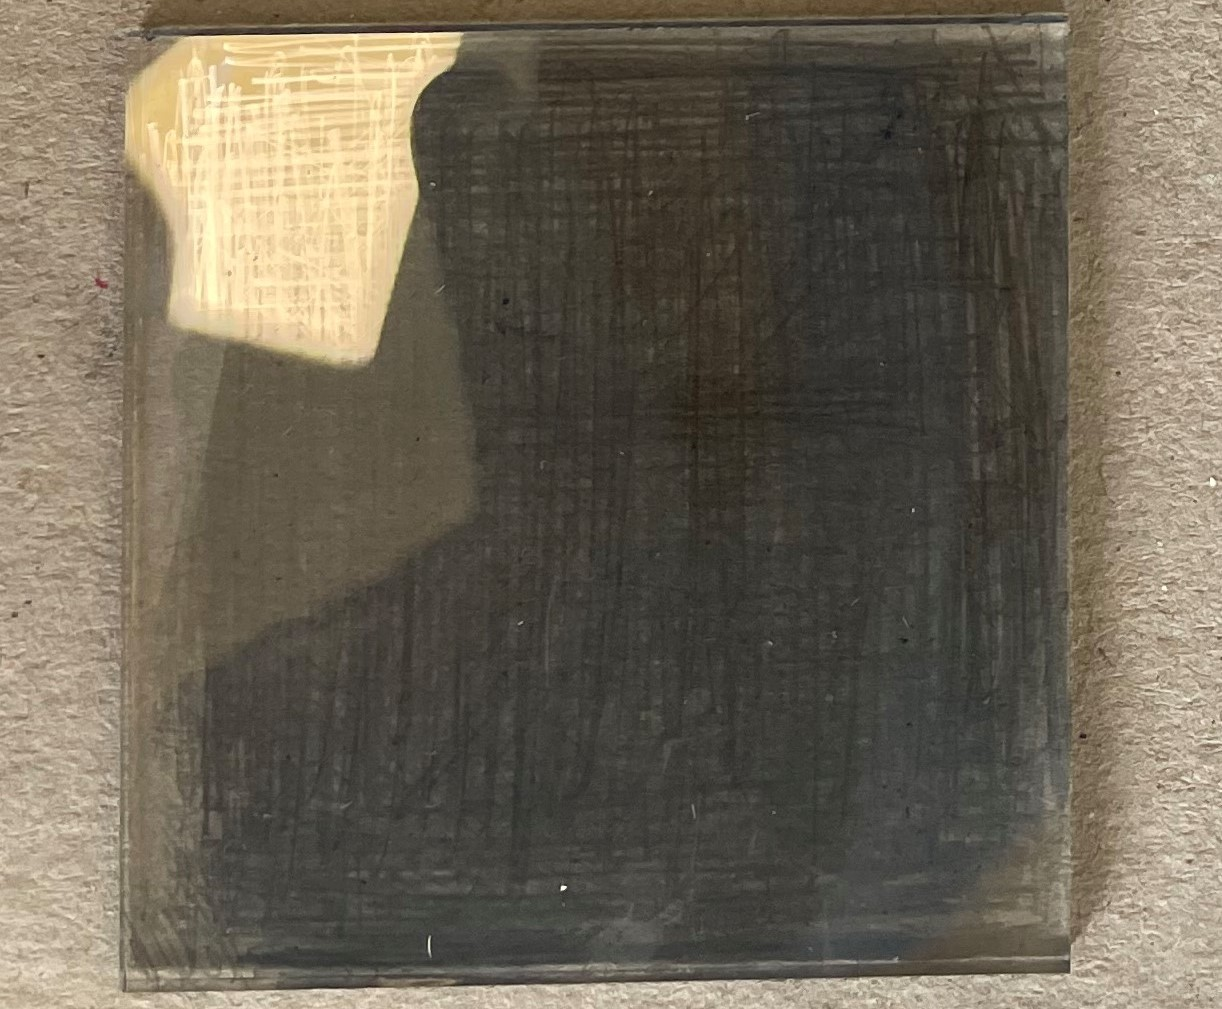
\includegraphics[width=\textwidth]{final_anode.jpg}
\caption{The final anode used, created by utilizing the graphite pencil.}
\label{fig:finalanode}
\end{figure}

\newpage

\subsection{Battery Evaluation Process}
\subsubsection{Experiment Design}
Throughout the construction process, the effectiveness of the individual components are assessed by different means. However, the final battery produced is evaluated according to three different discharge curves measured on two different batteries.
The curves are determined by connecting the charged battery to a constant load and measuring the current and the voltage over a period of time with a multimeter. 
A detailed circuit diagram can be seen in Fig. \ref{fig:circuitfig}. 
Three different discharge curves are measured. Two after a \SI{10}{\minute} charge with a \SI{1e3}{\ohm} resistor and a \SI{1e2}{\ohm} resistor respectively and the third after a \SI{20}{\minute} charge with a \SI{1e3}{\ohm} resistor. A recording period of 10 minutes is chosen, since the obtained values quickly fall below a significant value and a longer measuring period would be redundant.

\subsubsection{Variables}
\begin{table}[h]
\renewcommand{\arraystretch}{1.3}
\caption{Iteration Parameters}
\label{table:parametersbatteryevaluation}
\centering
\begin{tabular}{l|l|l||l}
\multicolumn{3}{c||}{\bfseries Parameter}&\bfseries Values\\
\hline
\hline
\multicolumn{2}{c|}{\multirow{3}{*}{Constant}}&The batteries utilized&Constructed as described above\\
\cline{3-4}
\multicolumn{2}{c|}{}&The charging voltage&\SI{4.6}{\volt}\\
\cline{3-4}
\multicolumn{2}{c|}{}&The discharge temperature&Room temperature (\SI{20}{\degreeCelsius})\\
\hline\hline
\multirow{2}{*}{Varying}&\multirow{2}{*}{Independent}&The discharge load&\SI{1e2}{\ohm} and \SI{1e3}{\ohm}\\
\cline{3-4}
&&The charge time&\SI{10}{\minute} and \SI{20}{\minute}\\
\cline{2-4}
&\multirow{2}{*}{Dependent}&The discharge current over time&To be measured\\
\cline{3-4}
&&The discharge voltage over time&To be measured\\
\end{tabular}
\end{table}

\begin{figure}[ht!]
\centering
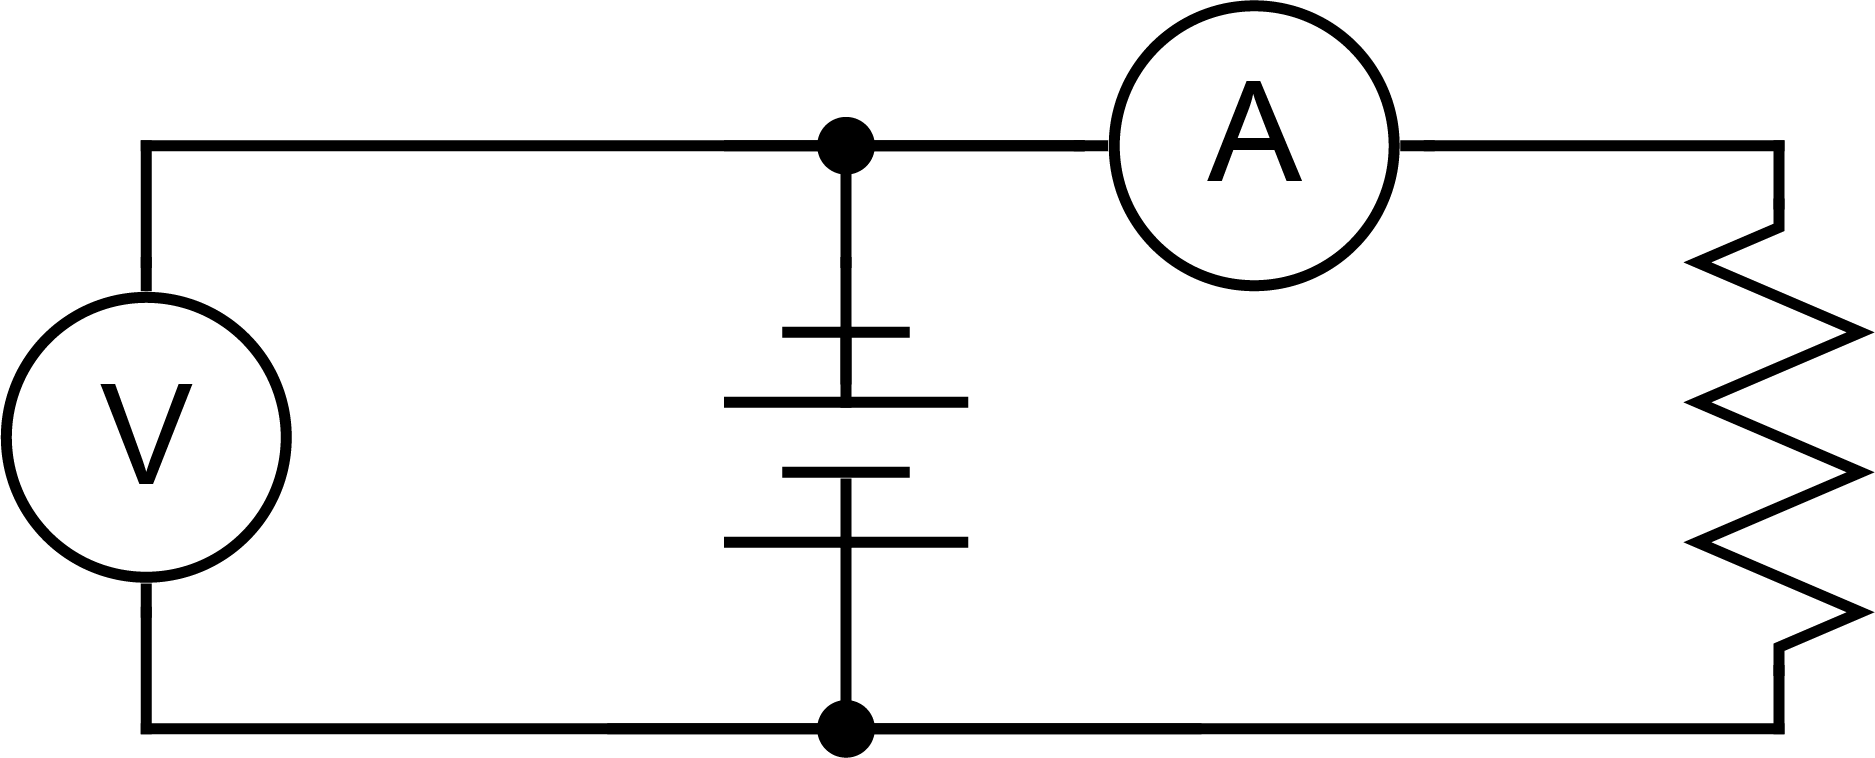
\includegraphics[width=\textwidth]{circuit.png}
\caption{The circuit used to measure the discharge curves.}
\label{fig:circuitfig}
\end{figure}

\newpage
    
\subsubsection{Process}
\begin{enumerate}
\item The battery is constructed and charged for \SI{10}{\minute} at a constant voltage of \SI{4.6}{\volt}.
\item The battery is then connected to the above described measuring circuit with a \SI{1e3}{\ohm} resistor and left to discharge for \SI{10}{\minute}.
\item The battery is recharged for \SI{10}{\minute} at a constant voltage of \SI{4.6}{\volt}.
\item It is again connected to the measuring circuit and discharged over a \SI{1e2}{\ohm} resistor for \SI{10}{\minute}.
\item The battery is recharged for \SI{20}{\minute} at a constant voltage of \SI{4.6}{\volt}.
\item The discharge curve is measured with a \SI{1e3}{\ohm} resistor for \SI{10}{\minute}.
\item This process is repeated for the second battery
\end{enumerate}

\subsection{Other Experiments}
The titanium-dioxide powder used was evaluated, since the origin of the powder initially utilized was unknown and thus considered a potential limitation. However, it was concluded, that the powder used initially, labelled with \textit{Degussa}, is the most suited for the task.

\begin{figure}[ht!]
\centering
\includegraphics[width=\textwidth]{different_titanium_dioxide_powder.png}
\caption{The different titanium-dioxide powders investigated.}
\label{fig:otherexp}
\end{figure}

The sodium-perchlorate concentration was investigated by creating three different batteries as per the method described above. They were filled with a \SI{0.2}{\mol\per\L}, a \SI{0.5}{\mol\per\L} and a \SI{1}{\mol\per\L} sodium-perchlorate, de-ionized water solution respectively, which acts as the electrolyte. It was concluded that \SI{1}{\mol\per\L} is the most effective electrolyte concentration. The evaluation of this experiment was out of scope of this investigation.

Two different battery form factors were evaluated. However, only a stack-based approach, with the electrodes being placed on top of one another and the electrolyte together with the tape separator in between, managed to function as a battery. The initial layout, as described in the reference experiment, suffered from various limitations\cite{Klaus2022}.

\begin{figure}[ht!]
\centering
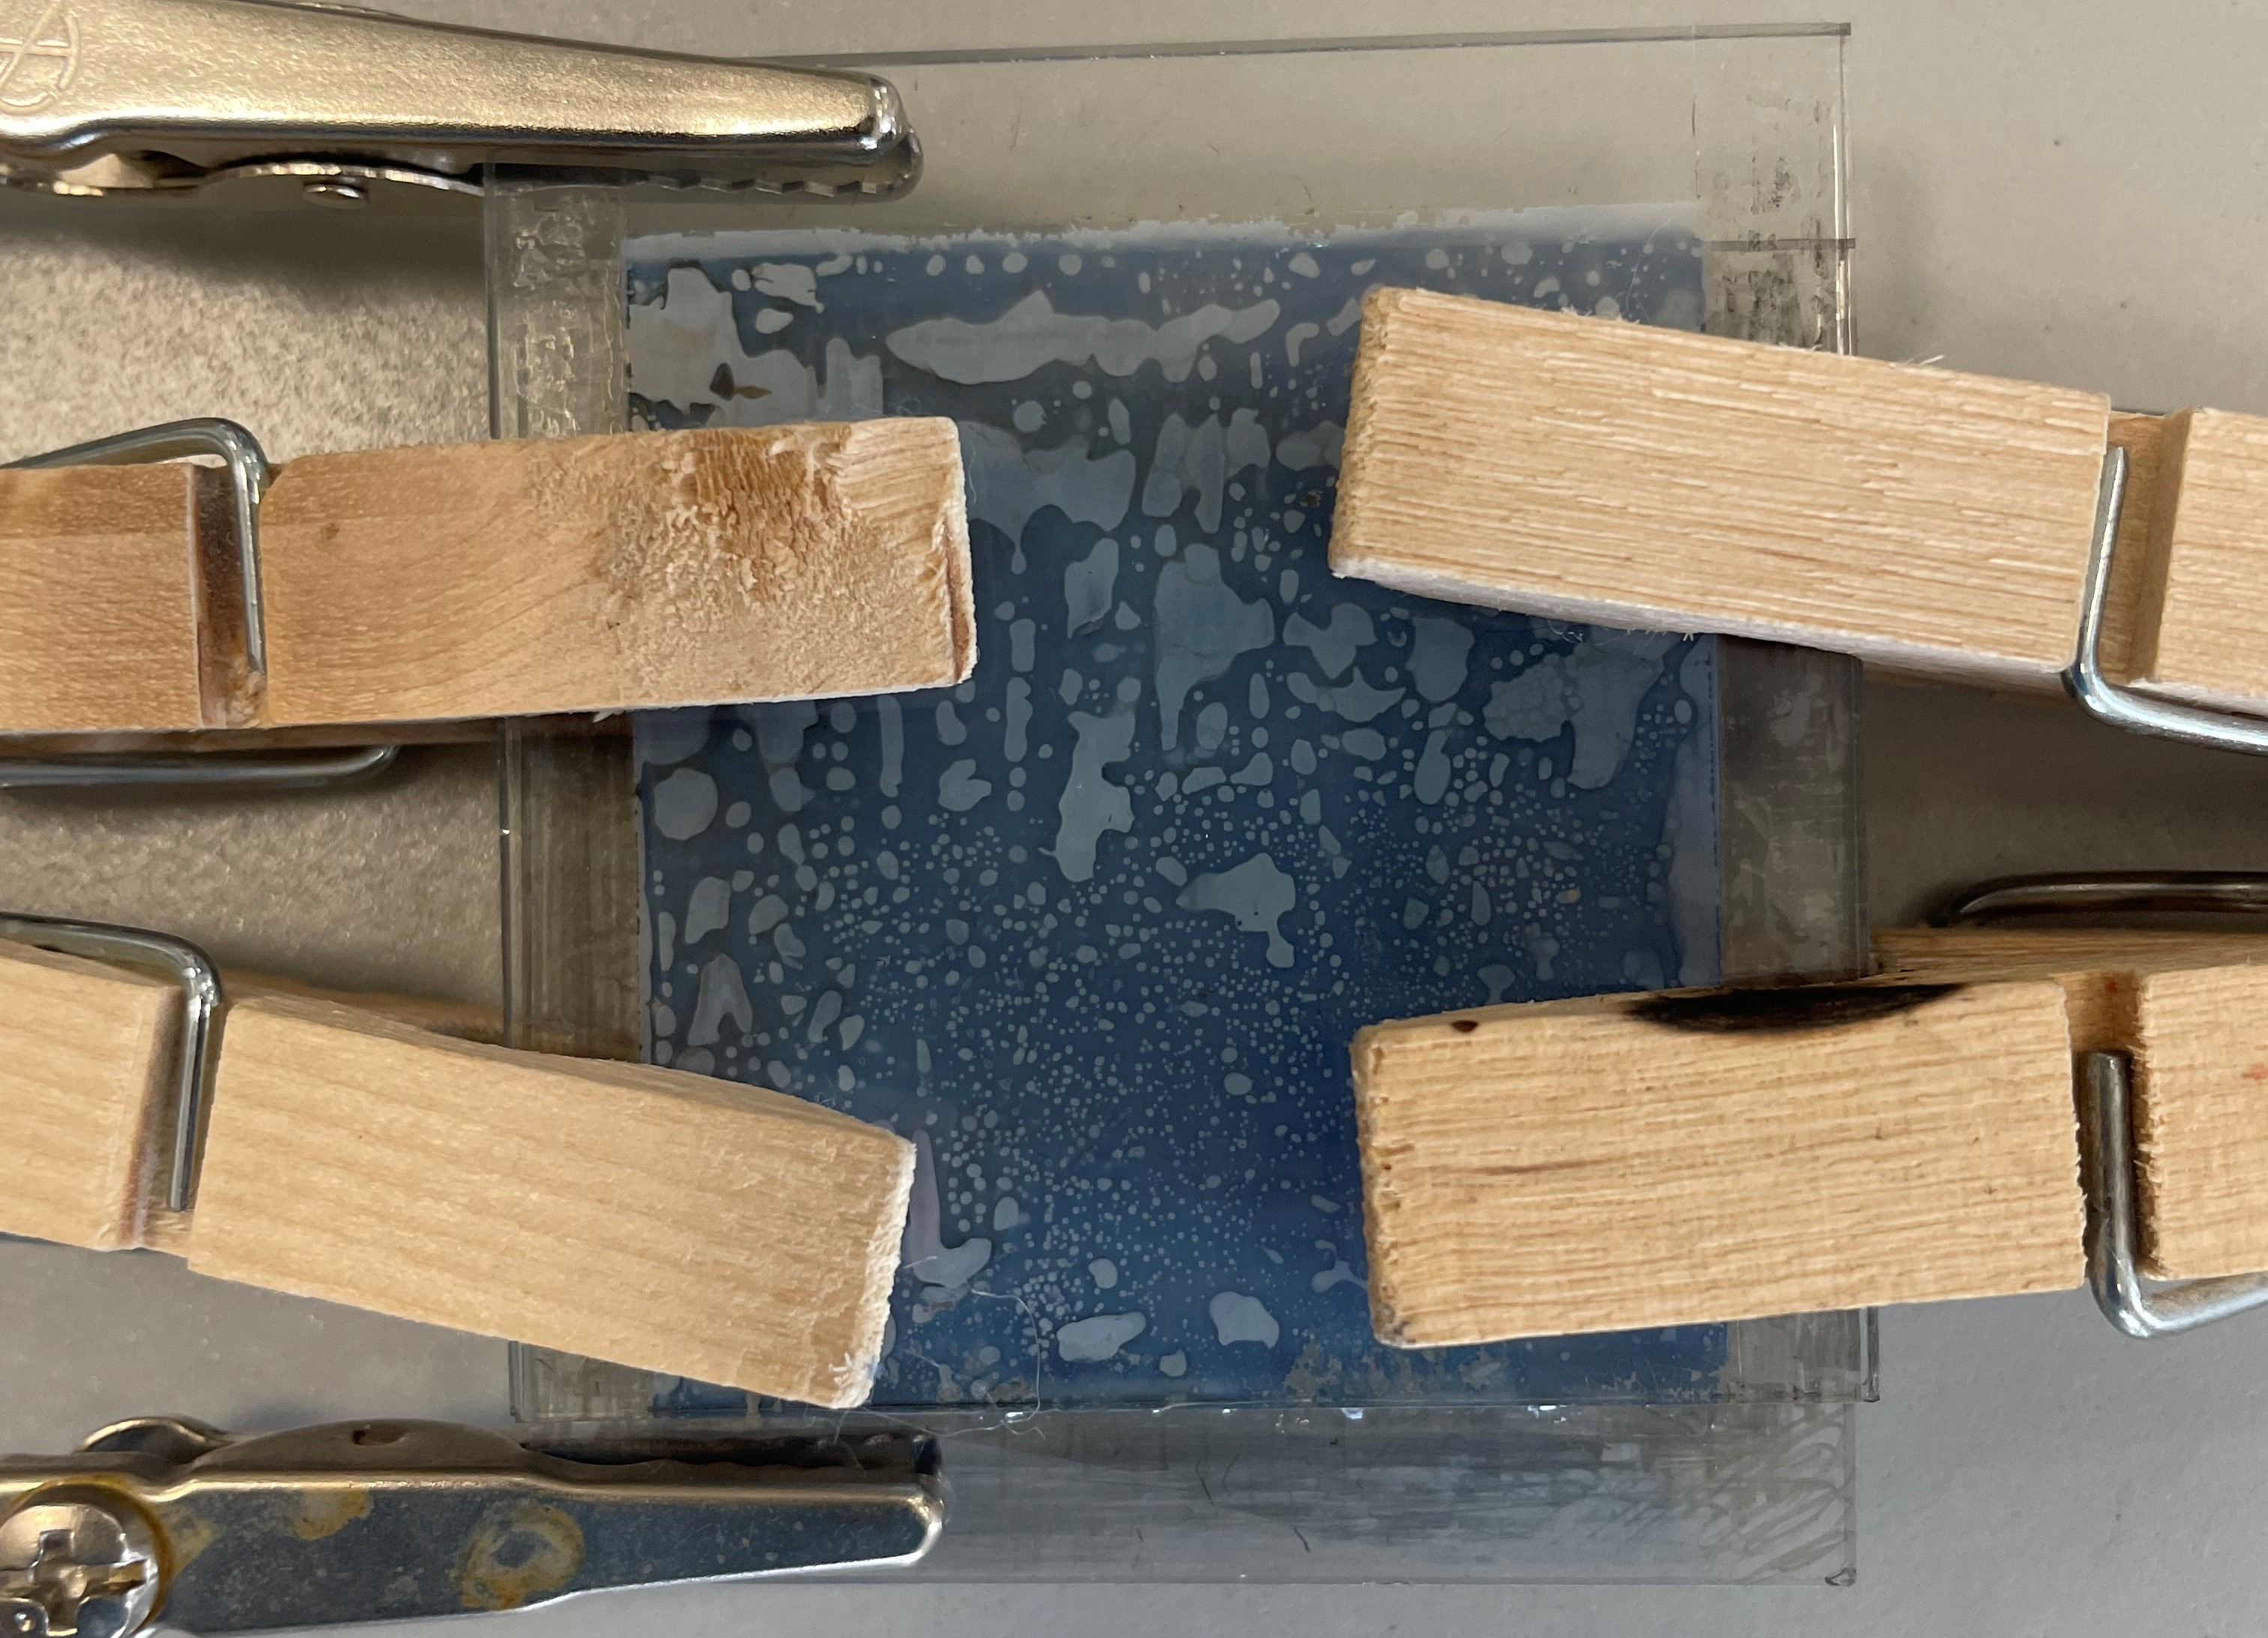
\includegraphics[width=\textwidth]{final_setup.jpg}
\caption{The stack-based battery form factor.}
\label{fig:finalsetup}
\end{figure}